\chapter{Vector Calculus}
\section{Vector Fields}
\begin{definition}[Vector Field]
    Let \(S \subseteq \mathbb{R} ^n\). A vector field is a vector-valued function \(\mathbf{F}(x_1,\ldots,x_n)\) where
    \[
        \mathbf{F}:S\to \mathbb{R}^n
    \]
    defined in terms of scalar-valued components.
\end{definition}
In calc 3, we work exclusively in terms of \(\mathbb{R}^2\) and \(\mathbb{R} ^3\) in this section, however I have made my above definition a bit more general. Examples and further definitions will all be on \(\mathbb{R} ^2\) or \(\mathbb{R} ^3\).\\
An example of a vector field is the function 
\[
    \mathbf{F} (x,y)=\left\langle \cos (xy),x^2 y^2 e^{xy\sin x}  \right\rangle
\]
because for any \((x,y\in\mathbb{R}^2)\), it takes on some value \(\mathbf{F}(x,y)\in\mathbb{R}^2\).
\begin{definition}[Component Functions]
    For a vector field defined as either 
    \[
        \mathbf{F}(x,y) =P(x,y)\hati +Q(x,y)\hatj
    \]
    or
    \[
        \mathbf{F}(x,y,z)=P(x,y,z)\hati+Q(x,y,z)\hatj+R(x,y,z)\hatk
    \]
    where \(P,Q,R\) are scalar valued functions, we say that \(P,Q,R\) are the component functions of \(\mathbf{F} \).
\end{definition}
\begin{remark}
    For some scalar valued \(f:\mathbb{R} ^2 \to \mathbb{R} \) or \(f:\mathbb{R}^3 \to \mathbb{R} \), the gradient vector \(\nabla f\) is really a vector field, defined as 
    \[
        \nabla f = f_x\hati +f_y\hatj
    \]
    or for \(f:\mathbb{R} ^3\to \mathbb{R} \),
    \[
        \nabla f = f_x\hati+f_y\hatj+f_z\hatk
    \]
\end{remark}
\begin{definition}[Conservative Vector Fields and Potential Function]
    Let \(\mathbf{F} \) be a vector field. We say that \(\mathbf{F} \) is a \textbf{conservative} \textbf{vector} \textbf{field} if and only if there exists some scalar valued \(f\) such that
    \[
        \mathbf{F} =\nabla f
    \]
    In this case, we say \(f\) is the \textbf{potential} \textbf{function} of \(\mathbf{F} \).
\end{definition}
Plotting vector fields by hand is hard, and is best left to computers. Here's an example done with TikZ:
\begin{center}
    Vector field for \(\mathbf{F}(x,y)= -y\hati +x\hatj\)\\
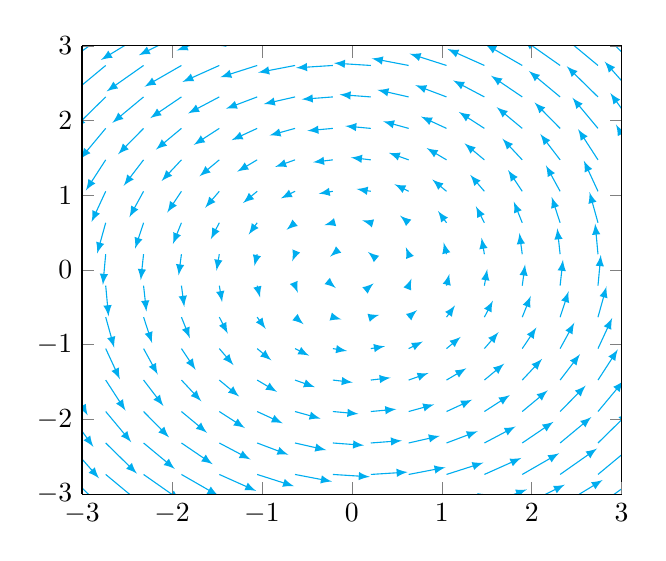
\begin{tikzpicture}
    \begin{axis}[
            view     = {0}{90}, % for a view 'from above'
            xmin=-3, xmax=3,
            ymin=-3, ymax=3,
            xtick    = {-3,...,3},
            ytick    = {-3,...,3},
        ]
        \addplot3[cyan, quiver={u=-y, v=x, scale arrows=0.15}, samples=20, domain=-4:4, y domain=-4:4, -latex] (x,y,0);
    \end{axis}
\end{tikzpicture}
\end{center}